\documentclass[11pt,a4paper]{article}
\usepackage[utf8]{inputenc}
\usepackage[margin=0.8in]{geometry}
\usepackage{hyperref}
\hypersetup{
    colorlinks=true,
    linkcolor=blue!80!black,
    citecolor=blue!80!black,
    urlcolor=cyan!80!black,
    pdftitle={EE8203 Department-Level Campus Network Design Technical Report},
    pdfauthor={Faculty of Engineering, University of Ruhuna}
}
\usepackage{amsmath,amssymb}
\usepackage{graphicx}
\usepackage{booktabs}
\usepackage{tabularx}
\usepackage{longtable}
\usepackage{array}
\usepackage{listings}
\usepackage{xcolor}
\usepackage{fancyhdr}
\usepackage{enumitem}
\usepackage{caption}

% Custom Horizontal Rule
\newcommand{\hr}{\vspace{0.2cm}\noindent\hrulefill\vspace{0.2cm}}

% Custom Column Types for Tabularx
\newcolumntype{L}{>{\raggedright\arraybackslash}X}
\newcolumntype{C}{>{\centering\arraybackslash}X}
\newcolumntype{R}{>{\raggedleft\arraybackslash}X}

% Pass/Fail Formatting using standard amssymb symbols
\newcommand{\cmark}{\textcolor{green!60!black}{\textbf{$\checkmark$}~PASS}}
\newcommand{\xmark}{\textcolor{red!70!black}{\textbf{$\times$}~FAIL}}

% Listing Styles
\definecolor{codebg}{RGB}{248, 249, 250}
\definecolor{codeframe}{RGB}{210, 215, 220}
\definecolor{commentgreen}{RGB}{34, 139, 34}
\definecolor{keywordblue}{RGB}{0, 51, 153}
\definecolor{stringred}{RGB}{163, 21, 21}

\lstdefinestyle{ciscostyle}{
    backgroundcolor=\color{codebg},
    basicstyle=\ttfamily\footnotesize,
    breakatwhitespace=false,
    breaklines=true,
    captionpos=b,
    commentstyle=\color{commentgreen},
    frame=single,
    rulecolor=\color{codeframe},
    keepspaces=true,
    keywordstyle=\color{keywordblue}\bfseries,
    showspaces=false,
    showstringspaces=false,
    showtabs=false,
    tabsize=2
}

\lstdefinestyle{pythonstyle}{
    language=Python,
    backgroundcolor=\color{codebg},
    basicstyle=\ttfamily\footnotesize,
    breakatwhitespace=false,
    breaklines=true,
    commentstyle=\color{commentgreen}\itshape,
    frame=single,
    rulecolor=\color{codeframe},
    keywordstyle=\color{keywordblue}\bfseries,
    stringstyle=\color{stringred},
    keepspaces=true,
    tabsize=4
}

\lstdefinestyle{yamlstyle}{
    backgroundcolor=\color{codebg},
    basicstyle=\ttfamily\footnotesize,
    breaklines=true,
    frame=single,
    rulecolor=\color{codeframe},
    commentstyle=\color{commentgreen}\itshape,
    keywordstyle=\color{keywordblue}\bfseries,
    stringstyle=\color{stringred}
}

\lstdefinestyle{console}{
    backgroundcolor=\color{codebg},
    basicstyle=\ttfamily\scriptsize,
    breaklines=true,
    frame=single,
    rulecolor=\color{codeframe}
}

\pagestyle{fancy}
\fancyhf{}
\renewcommand{\headrulewidth}{0pt}
\rfoot{\thepage}

\begin{document}

% Cover Page / Title Page Layout matching University of Ruhuna format
\begin{titlepage}
\centering
\thispagestyle{empty}

\vspace*{0.4cm}


\includegraphics[width=3.0cm]{images/ruhuna_logo.png}

\vfill

{\LARGE \textbf{Department-Level Campus Network Design, Multi-Layer Routing, Security Policy Enforcement, Dual-Tier Automation \& Monitoring}}\\[0.6cm]
{\large \textbf{EE8203 — Design and Management of Data Networks}}

\vfill

{\large A project report submitted to the}

\vfill

{\Large Department of Electrical and Information Engineering}\\[0.25cm]
{\Large Faculty of Engineering}\\[0.25cm]
{\Large University of Ruhuna}\\[0.25cm]
{\Large Sri Lanka}

\vfill

{\large in partial fulfillment of the requirements for the}

\vfill

{\Large \textbf{Degree of the Bachelor of the Science of Engineering Honours}}

\vfill

{\large by}

\vspace{0.4cm}

% Group Members Table - Modify or add members here:
\begin{tabular}{lcl}
Panditha T.N. & - & EG/2021/4702 \\
Rathnayaka R.M.K.D. & - & EG/2021/4758 \\
Wijesinghe D.M.A.B. & - & EG/2021/4875 \\
\end{tabular}

\vspace*{1.2cm}

\end{titlepage}
\newpage

\noindent
\begin{table}[htbp]
\centering
\begin{tabular}{|p{0.25\textwidth}|p{0.68\textwidth}|}
\hline
\textbf{Document Metadata} & \textbf{Details} \\
\hline
\textbf{Module} & EE8203 -- Design and Management of Data Networks \\
\textbf{Institution} & Dept. of Electrical \& Information Engineering, Faculty of Engineering, Univ. of Ruhuna \\
\textbf{Project Title} & Dept-Level Campus Network Design, Multi-Layer Routing, Security Policy, Dual-Tier Automation \& Monitoring \\
\textbf{Date of Submission} & August 2026 \\
\textbf{Target Infrastructure} & GNS3 Simulation Engine (Cisco IOSv / IOSvL2 / Cisco 7200 / Ubuntu Linux VMs) \\
\textbf{Document Version} & 1.0 (Final Technical Report) \\
\hline
\end{tabular}
\end{table}

\hr

\section{Executive Summary}

This report documents the end-to-end design, implementation, security policy enforcement, multi-tier network automation, and real-time monitoring of a modern department-level campus network for the Hapugala premises of the Faculty of Engineering, University of Ruhuna. The network interconnects four primary departments: Electrical \& Information Engineering (\textbf{DEIE}), Civil \& Environmental Engineering (\textbf{DCEE}), Mechanical \& Manufacturing Engineering (\textbf{DMME}), and Inter-Disciplinary Studies (\textbf{DIS}).

To fulfill the rigorous requirements of high availability, security segmentation, scalability, and ease of management, the infrastructure was engineered following Cisco's \textbf{Three-Layer Hierarchical Network Model} (Core, Distribution, and Access layers). A key architectural evolution detailed in this report is the transition of the distribution layer from a traditional Layer 2 trunking topology to a \textbf{Layer 3 Multilayer Distribution Architecture}. By terminating Virtual Local Area Networks (VLANs) at local distribution switches (\textbf{SW-D-DEIE}, \textbf{SW-D-DCEE}, \textbf{SW-D-DMME}) and utilizing \texttt{/30} point-to-point routed uplinks with \textbf{Open Shortest Path First (OSPF Area 0)} dynamic routing to the core switch (\textbf{SW-CORE}), Spanning Tree Protocol (STP) loops across the core backbone are eliminated, convergence time is reduced to sub-seconds, and bandwidth utilization is optimized.

Inter-departmental security policies are enforced strictly using \textbf{Extended Named Access Control Lists (ACLs)} applied inbound on Distribution SVIs and Core interfaces. The implemented policy grants full bidirectional server farm access to DEIE engineering workstations, limits DCEE administrative staff to web services (HTTP/HTTPS) in DIS while blocking ping/ICMP, completely isolates the DMME workshop lab from all external academic subnets, and allows return-established TCP sessions while denying unauthorized inbound connections. Reachability compliance is rigorously verified using a complete \textbf{\texorpdfstring{$4 \times 4$}{4x4} Department Reachability Test Matrix}, providing detailed ping and traceroute evidence alongside ACL match counter verification.

To eliminate manual configuration errors and ensure operational repeatability, a \textbf{Dual-Tier Network Automation Framework} was constructed:
\begin{enumerate}
    \item \textbf{Python with Netmiko}: Used for imperative control, interface provisioning, OSPF configuration, NAT rules, and SNMP community string pushes across core and edge routers (\textbf{R-CORE}, \textbf{R-EDGE}).
    \item \textbf{Ansible (Cisco IOS Collection)}: Used for declarative state management, role-based modular configuration (\texttt{vlans}, \texttt{trunking}, \texttt{access\_ports}, \texttt{stp}, \texttt{l3\_distribution}, \texttt{l2\_gateway}), idempotency verification via \texttt{--check}, and automated rollback capabilities across all 7 switches.
\end{enumerate}

Finally, continuous enterprise monitoring is established via a \textbf{Zabbix 6.x LTS} platform deployed on an Ubuntu Linux virtual machine (\textbf{VM-ZABBIX}). Routers and switches are onboarded via SNMPv2c using standard Cisco templates. Custom triggers are configured for ICMP outages, interface down transitions, high CPU utilization, and management plane reachability split protections. The system features a customized dashboard (\texttt{FoE-UoR Network}) providing real-time visibility into campus link health, host availability, and active alert counters.

\hr

\section{Campus Network Design \& Architecture}

\subsection{Topology Architecture Overview}

The campus network is structured around a three-tier hierarchical architecture designed to separate core routing, distribution-level aggregation, and access-layer host connectivity:

\begin{figure}[htbp]
\centering
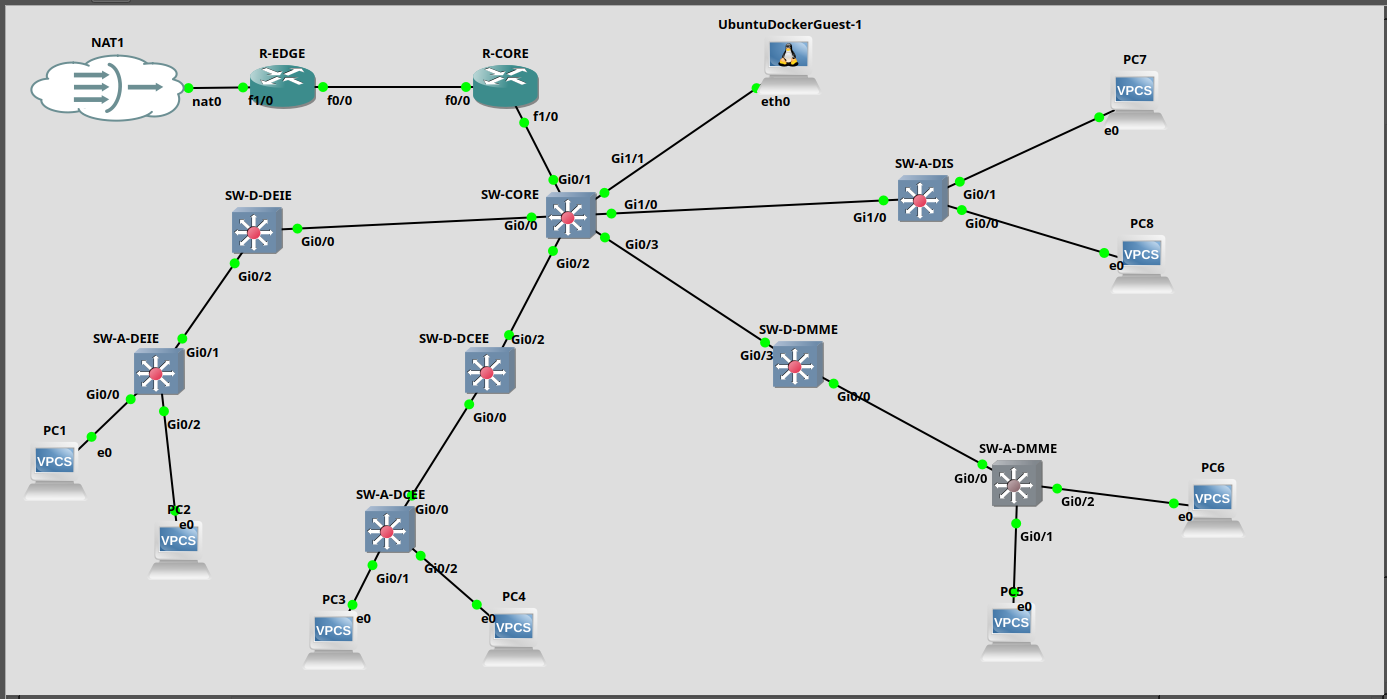
\includegraphics[width=0.88\textwidth]{images/topology.png}
\caption{GNS3 Network Simulation Topology Diagram illustrating the 3-Tier Architecture, IP Address Allocation, and Interconnections}
\label{fig:topology}
\end{figure}

\begin{lstlisting}[style=console, caption={Campus Network Three-Tier Hierarchical Schematic}]
                          [ Internet Cloud ]
                                  |
                              (Gi0/0)
                           [ R-EDGE ] (10.0.0.1/30)
                                  |
                              (Gi0/1)
                                  |
                              (Gi0/1)
                           [ R-CORE ] (10.0.1.1/30)
                                  |
                              (Gi0/0)
                                  |
                              (Gi0/1)
                          [ SW-CORE ] (Core L3 Switch)
             +--------------------+--------------------+
       (Gi0/2) 10.0.10.1/30 (Gi0/3) 10.0.20.1/30 (Gi0/4) 10.0.30.1/30
             |                    |                    |
          (Gi0/0)              (Gi0/2)              (Gi0/3)
      [ SW-D-DEIE ]        [ SW-D-DCEE ]        [ SW-D-DMME ]
   (Dist L3 - VLAN 10)  (Dist L3 - VLAN 20)  (Dist L3 - VLAN 30)
             |                    |                    |
        (L2 Trunk)           (L2 Trunk)           (L2 Trunk)
             |                    |                    |
      [ SW-A-DEIE ]        [ SW-A-DCEE ]        [ SW-A-DMME ]
     (Access L2)          (Access L2)          (Access L2)
       +-----+---+          +-----+---+          +-----+---+
     (PC1)       (PC2)    (PC3)       (PC4)    (PC5)       (PC6)
    VLAN 10     VLAN 10  VLAN 20     VLAN 20  VLAN 30     VLAN 30
    
   * Note: SW-A-DIS (Access L2, VLAN 40) trunks directly to SW-CORE (Gi1/0).
   * VM-AUTO (10.99.99.100) and VM-ZABBIX (10.10.40.100) connect to SW-CORE.
\end{lstlisting}

\subsection{Network Inventory \& Device Selection Justification}

The network infrastructure comprises 13 active configurable devices and multiple end-user hosts, detailed in Table~\ref{tab:inventory}.

\begin{table}[htbp]
\centering
\caption{Network Inventory and Device Selection Rationale}
\label{tab:inventory}
\scriptsize
\begin{tabularx}{\textwidth}{@{}l p{1.3cm} p{1.8cm} p{2.4cm} L@{}}
\toprule
\textbf{Hostname} & \textbf{Category} & \textbf{GNS3 Image} & \textbf{Primary OSI Role} & \textbf{Justification \& Rationale} \\
\midrule
\textbf{R-EDGE} & WAN Gateway & Cisco 7200 (IOS 15.2) & Layer 3 Edge Gateway / PAT / Static Route & Connects campus to ISP; handles Network Address Translation (NAT Overload) restricting external access to authorized subnets (DEIE \& DCEE). \\
\midrule
\textbf{R-CORE} & Core Router & Cisco 7200 (IOS 15.2) & Layer 3 Core Routing \& Transit & High-throughput internal routing backbone interconnecting WAN Edge with Campus LAN; runs OSPF Area 0. \\
\midrule
\textbf{SW-CORE} & Core Switch & IOSvL2 Multilayer & Layer 3 Backbone \& DIS Gateway & Provides high-speed inter-switch transit, anchors DIS Server Farm (VLAN 40), and runs OSPF Area 0 across routed uplinks. \\
\midrule
\textbf{SW-D-DEIE} & Distribution & IOSvL2 Multilayer & Layer 3 DEIE Gateway \& Aggregation & Terminates VLAN 10 SVI, performs local routing for DEIE, eliminates STP loops over core uplink, enforces local ACLs. \\
\midrule
\textbf{SW-D-DCEE} & Distribution & IOSvL2 Multilayer & Layer 3 DCEE Gateway \& Aggregation & Terminates VLAN 20 SVI, routes DCEE administrative traffic, and enforces HTTP/HTTPS-only security constraints. \\
\midrule
\textbf{SW-D-DMME} & Distribution & IOSvL2 Multilayer & Layer 3 DMME Gateway \& Aggregation & Terminates VLAN 30 SVI, routes DMME workshop traffic, and enforces total isolation ACL policies. \\
\midrule
\textbf{SW-A-DEIE} & Access Switch & IOSvL2 L2 Switch & Layer 2 Host Access (DEIE) & Connects DEIE workstations (PC1, PC2), enforces port-security/STP portfast, trunks to SW-D-DEIE over 802.1Q. \\
\midrule
\textbf{SW-A-DCEE} & Access Switch & IOSvL2 L2 Switch & Layer 2 Host Access (DCEE) & Connects DCEE admin PCs (PC3, PC4), provisions VLAN 20 access ports, trunks to SW-D-DCEE. \\
\midrule
\textbf{SW-A-DMME} & Access Switch & IOSvL2 L2 Switch & Layer 2 Host Access (DMME) & Connects DMME workshop PCs (PC5, PC6), provisions VLAN 30 access ports, trunks to SW-D-DMME. \\
\midrule
\textbf{SW-A-DIS} & Access Switch & IOSvL2 L2 Switch & Layer 2 Host/Server Access (DIS) & Connects DIS server farm and workstations (PC7, PC8, Zabbix VM), trunks directly to SW-CORE. \\
\midrule
\textbf{VM-AUTO} & Control Server & Ubuntu 22.04 Container & Network Automation Host & Hosted on VLAN 99 (\texttt{10.99.99.100}); runs Python/Netmiko scripts and Ansible playbooks via SSH. \\
\midrule
\textbf{VM-ZABBIX} & Monitoring & Ubuntu 22.04 VM & Network Management System (NMS) & Hosted on VLAN 40 (\texttt{10.10.40.100}); polls SNMPv2c metrics and ICMP health from all campus switches/routers. \\
\midrule
\textbf{VM-DHCP/WEB} & App Server & Linux Container/VM & Web \& Reachability Testing & Hosts HTTP/HTTPS services in DIS (VLAN 40) for policy verification. \\
\midrule
\textbf{VPC Hosts} & End Stations & GNS3 VPCS (8+ units) & Host Simulation \& ACL Testing & Two VPCs per department (PC0/PC1, PC3/PC6, PC4/PC5, DIS-PC) used for matrix ping testing. \\
\bottomrule
\end{tabularx}
\end{table}

\subsubsection{Architectural Justification of Layer 3 Distribution Conversion}
Initially, distribution switches functioned as pure Layer 2 bridges, extending VLAN 10, 20, 30, and 99 trunks back to \textbf{SW-CORE}. This traditional design presented severe operational drawbacks:
\begin{enumerate}
    \item \textbf{STP Loop Vulnerabilities}: Spanning Tree Protocol had to block duplicate links between switches, leaving bandwidth unused and risking campus-wide broadcast storms if STP failed.
    \item \textbf{Sub-Optimal Gateway Routing}: Inter-VLAN traffic had to traverse Layer 2 trunks to SW-CORE for routing, increasing latency and backbone utilization.
    \item \textbf{VLAN 99 L2 Fragmentation Risk}: Converting distribution switch uplinks to Layer 3 \texttt{/30} routed ports separated VLAN 99 into distinct Layer 2 domains, necessitating explicit Layer 3 host routes (\texttt{/32}) on SW-CORE to preserve management plane reachability to all nodes.
\end{enumerate}

By moving default gateways (SVIs) down to \textbf{SW-D-DEIE}, \textbf{SW-D-DCEE}, and \textbf{SW-D-DMME}, Layer 2 broadcasts are constrained to local access switches. Uplinks to SW-CORE operate as point-to-point Layer 3 links (\texttt{no switchport}), enabling equal-cost multipath routing and sub-second OSPF reconvergence.

\subsection{VLAN Allocation and IP Addressing Scheme}

The campus network uses the private \texttt{10.0.0.0/8} IP address block, structured systematically into departmental client subnets, management subnets, and point-to-point \texttt{/30} routed links.

\begin{table}[htbp]
\centering
\caption{Departmental VLAN \& Subnet Allocation}
\label{tab:vlans}
\small
\begin{tabularx}{\textwidth}{@{}c l l l l L@{}}
\toprule
\textbf{VLAN} & \textbf{VLAN Name} & \textbf{Department / Zone} & \textbf{Subnet} & \textbf{Gateway SVI} & \textbf{Purpose \& Egress Policy} \\
\midrule
\textbf{10} & \texttt{VLAN\_DEIE} & Electrical \& Info Eng. & \texttt{10.10.10.0/24} & \texttt{10.10.10.1} & Workstations \& labs; full internet \& server farm access. \\
\textbf{20} & \texttt{VLAN\_DCEE} & Civil \& Env. Eng. & \texttt{10.10.20.0/24} & \texttt{10.10.20.1} & Admin \& project offices; internet \& DIS web access only. \\
\textbf{30} & \texttt{VLAN\_DMME} & Mech. \& Mfg. Eng. & \texttt{10.10.30.0/24} & \texttt{10.10.30.1} & Workshop labs; fully isolated from other departmental subnets. \\
\textbf{40} & \texttt{VLAN\_DIS} & Inter-Disciplinary & \texttt{10.10.40.0/24} & \texttt{10.10.40.1} & Central IT Server Farm \& Zabbix NMS; accessible by DEIE/DCEE. \\
\textbf{99} & \texttt{MGMT} & Infrastructure & \texttt{10.99.99.0/24} & \texttt{10.99.99.1} & Out-of-band management plane (SSH, SNMP, Ansible, Netmiko). \\
\textbf{100} & \texttt{NATIVE} & Trunk Interfaces & N/A & N/A & Security baseline for untagged trunk frames (unused native VLAN). \\
\bottomrule
\end{tabularx}
\end{table}

\begin{table}[htbp]
\centering
\caption{Point-to-Point Layer 3 Link Table}
\label{tab:p2p}
\small
\begin{tabularx}{\textwidth}{@{}l l l c c c@{}}
\toprule
\textbf{Link Segment} & \textbf{Source Device \& Port} & \textbf{Destination Device \& Port} & \textbf{Subnet Prefix} & \textbf{Source IP} & \textbf{Dest IP} \\
\midrule
\textbf{R-EDGE $\leftrightarrow$ R-CORE} & R-EDGE (\texttt{Gi0/1}) & R-CORE (\texttt{Gi0/1}) & \texttt{10.0.0.0/30} & \texttt{10.0.0.1} & \texttt{10.0.0.2} \\
\textbf{R-CORE $\leftrightarrow$ SW-CORE} & R-CORE (\texttt{Gi0/0}) & SW-CORE (\texttt{Gi0/1}) & \texttt{10.0.1.0/30} & \texttt{10.0.1.1} & \texttt{10.0.1.2} \\
\textbf{SW-CORE $\leftrightarrow$ SW-D-DEIE} & SW-CORE (\texttt{Gi0/2}) & SW-D-DEIE (\texttt{Gi0/0}) & \texttt{10.0.10.0/30} & \texttt{10.0.10.1} & \texttt{10.0.10.2} \\
\textbf{SW-CORE $\leftrightarrow$ SW-D-DCEE} & SW-CORE (\texttt{Gi0/3}) & SW-D-DCEE (\texttt{Gi0/2}) & \texttt{10.0.20.0/30} & \texttt{10.0.20.1} & \texttt{10.0.20.2} \\
\textbf{SW-CORE $\leftrightarrow$ SW-D-DMME} & SW-CORE (\texttt{Gi0/4}) & SW-D-DMME (\texttt{Gi0/3}) & \texttt{10.0.30.0/30} & \texttt{10.0.30.1} & \texttt{10.0.30.2} \\
\bottomrule
\end{tabularx}
\end{table}

\begin{table}[htbp]
\centering
\caption{Infrastructure Management IP Assignment Table}
\label{tab:mgmt_ips}
\small
\begin{tabularx}{\textwidth}{@{}l c c l c@{}}
\toprule
\textbf{Hostname} & \textbf{Management IP} & \textbf{Subnet Mask} & \textbf{Default Gateway} & \textbf{OSPF Router ID} \\
\midrule
\textbf{SW-CORE} & \texttt{10.99.99.1} & \texttt{255.255.255.0} & N/A (L3 Routing Enabled) & \texttt{1.1.1.1} \\
\textbf{SW-D-DEIE} & \texttt{10.99.99.11} & \texttt{255.255.255.0} & Host Route via \texttt{10.0.10.1} & \texttt{3.3.3.11} \\
\textbf{SW-D-DCEE} & \texttt{10.99.99.12} & \texttt{255.255.255.0} & Host Route via \texttt{10.0.20.1} & \texttt{3.3.3.12} \\
\textbf{SW-D-DMME} & \texttt{10.99.99.13} & \texttt{255.255.255.0} & Host Route via \texttt{10.0.30.1} & \texttt{3.3.3.13} \\
\textbf{SW-A-DEIE} & \texttt{10.99.99.21} & \texttt{255.255.255.0} & \texttt{10.99.99.11} (SW-D-DEIE) & N/A (L2 Only) \\
\textbf{SW-A-DCEE} & \texttt{10.99.99.22} & \texttt{255.255.255.0} & \texttt{10.99.99.12} (SW-D-DCEE) & N/A (L2 Only) \\
\textbf{SW-A-DMME} & \texttt{10.99.99.23} & \texttt{255.255.255.0} & \texttt{10.99.99.13} (SW-D-DMME) & N/A (L2 Only) \\
\textbf{SW-A-DIS} & \texttt{10.99.99.24} & \texttt{255.255.255.0} & \texttt{10.99.99.1} (SW-CORE) & N/A (L2 Only) \\
\bottomrule
\end{tabularx}
\end{table}

\subsection{Routing Architecture \& NAT Overload}

\subsubsection{Open Shortest Path First (OSPF Area 0)}
Dynamic interior routing is enabled across all Layer 3 nodes using single-area OSPF (\textbf{Area 0}). 
\begin{itemize}
    \item \textbf{Core Router (R-CORE)} advertises transit link \texttt{10.0.0.0/30} and backbone link \texttt{10.0.1.0/30}.
    \item \textbf{SW-CORE} advertises backbone link \texttt{10.0.1.0/30}, point-to-point links (\texttt{10.0.10.0/30}, \texttt{10.0.20.0/30}, \texttt{10.0.30.0/30}), server farm network \texttt{10.10.40.0/24}, and management subnet \texttt{10.99.99.0/24}.
    \item \textbf{Distribution Switches} advertise their respective routed \texttt{/30} links and client SVIs (\texttt{10.10.10.0/24}, \texttt{10.10.20.0/24}, \texttt{10.10.30.0/24}).
\end{itemize}
Passive interface commands (\texttt{passive-interface default}) are configured across OSPF processes, explicitly enabling only active transit links to prevent unauthorized OSPF neighbor adjacencies on client-facing SVIs.

\subsubsection{Static Default Routing \& Internet Egress}
A static default route is configured on \textbf{R-EDGE} pointing to the external ISP cloud:
\begin{lstlisting}[style=ciscostyle]
ip route 0.0.0.0 0.0.0.0 FastEthernet0/0 203.0.113.1
\end{lstlisting}
\textbf{R-CORE} receives a static default route pointing to \textbf{R-EDGE} (\texttt{10.0.0.1}), which is redistributed into OSPF via \texttt{default-information originate} on R-CORE, propagating a default route to SW-CORE and all distribution switches.

\subsubsection{Network Address Translation (PAT) Policy}
To enforce internet access policies, \textbf{R-EDGE} implements Port Address Translation (NAT Overload). In strict compliance with Section 3.3 of the project guidelines, \textbf{only DEIE (VLAN 10) and DCEE (VLAN 20) are granted internet egress}. DMME (VLAN 30) and DIS (VLAN 40) are denied internet translation.

\begin{lstlisting}[style=ciscostyle, caption={R-EDGE NAT ACL Configuration}]
! R-EDGE NAT ACL Configuration
ip access-list standard NAT_ALLOWED
 permit 10.10.10.0 0.0.0.255
 permit 10.10.20.0 0.0.0.255
 deny   ip any

ip nat inside source list NAT_ALLOWED interface FastEthernet0/0 overload

interface FastEthernet0/0
 ip nat outside

interface GigabitEthernet0/1
 ip nat inside
\end{lstlisting}

\hr

\section{Security Policy Implementation \& ACL Matrix}

\subsection{Extended Named ACL Specifications}

To enforce departmental security boundaries, extended named ACLs are deployed inbound on the respective Layer 3 switch SVI interfaces.

\begin{table}[htbp]
\centering
\caption{Extended Named ACL Specifications}
\label{tab:acls}
\small
\begin{tabularx}{\textwidth}{@{}l p{3.5cm} L L@{}}
\toprule
\textbf{ACL Name} & \textbf{Application Interface} & \textbf{Filtering Rules Summary} & \textbf{Policy Rationale} \\
\midrule
\texttt{ACL-DEIE-IN} & \texttt{SW-D-DEIE}\newline \texttt{interface vlan 10} (\texttt{in}) & 
• Permit IP \texttt{10.10.10.0/24} $\rightarrow$ \texttt{10.10.40.0/24}\newline
• Deny IP \texttt{10.10.10.0/24} $\rightarrow$ \texttt{10.10.20.0/24}\newline
• Deny IP \texttt{10.10.10.0/24} $\rightarrow$ \texttt{10.10.30.0/24}\newline
• Permit IP \texttt{10.10.10.0/24} $\rightarrow$ \texttt{any} & 
DEIE engineering staff have full access to DIS server farm and internet; blocked from probing DCEE/DMME. \\
\midrule
\texttt{ACL-DCEE-IN} & \texttt{SW-D-DCEE}\newline \texttt{interface vlan 20} (\texttt{in}) & 
• Permit TCP \texttt{10.10.20.0/24} $\rightarrow$ \texttt{10.10.40.0/24} (eq 80, 443)\newline
• Deny IP \texttt{10.10.20.0/24} $\rightarrow$ \texttt{10.10.40.0/24}\newline
• Deny IP \texttt{10.10.20.0/24} $\rightarrow$ \texttt{10.10.10.0/24}\newline
• Deny IP \texttt{10.10.20.0/24} $\rightarrow$ \texttt{10.10.30.0/24}\newline
• Permit IP \texttt{10.10.20.0/24} $\rightarrow$ \texttt{any} & 
DCEE admin staff are restricted to web services (HTTP/HTTPS) in DIS; ping (ICMP) to DIS is dropped; blocked from DEIE/DMME. \\
\midrule
\texttt{ACL-DMME-IN} & \texttt{SW-D-DMME}\newline \texttt{interface vlan 30} (\texttt{in}) & 
• Deny IP \texttt{10.10.30.0/24} $\rightarrow$ \texttt{10.10.10.0/24}\newline
• Deny IP \texttt{10.10.30.0/24} $\rightarrow$ \texttt{10.10.20.0/24}\newline
• Deny IP \texttt{10.10.30.0/24} $\rightarrow$ \texttt{10.10.40.0/24}\newline
• Deny IP \texttt{10.10.30.0/24} $\rightarrow$ \texttt{any} & 
DMME workshop lab is completely isolated from all other academic subnets and server farm zone. \\
\midrule
\texttt{ACL-DIS-IN} & \texttt{SW-CORE}\newline \texttt{interface vlan 40} (\texttt{in}) & 
• Permit IP \texttt{10.10.40.0/24} $\rightarrow$ \texttt{10.10.10.0/24}\newline
• Permit TCP \texttt{10.10.40.0/24} established $\rightarrow$ \texttt{10.10.20.0/24}\newline
• Deny IP \texttt{10.10.40.0/24} $\rightarrow$ \texttt{10.10.20.0/24}\newline
• Deny IP \texttt{10.10.40.0/24} $\rightarrow$ \texttt{10.10.30.0/24} & 
Permits return web traffic to DCEE; full access to DEIE; prohibits DIS initiated sessions to DCEE/DMME. \\
\midrule
\texttt{ACL-MGMT-IN} & \texttt{SW-CORE}\newline \texttt{interface vlan 99} (\texttt{in}) & 
• Permit SSH (TCP 22) from \texttt{10.99.99.0/24} to management IPs\newline
• Permit SNMP (UDP 161/162) to Zabbix Host (\texttt{10.10.40.100}) & 
Out-of-band management access is restricted strictly to SSH plane; SNMP metrics permitted to Zabbix host. \\
\bottomrule
\end{tabularx}
\end{table}

\subsection{\texorpdfstring{$4 \times 4$}{4x4} Department Reachability Test Matrix}

Comprehensive ICMP ping and traceroute testing was conducted across all 16 pair combinations of departmental endpoints:
\begin{itemize}
    \item \textbf{DEIE Test Host}: \texttt{PC0} (\texttt{10.10.10.10/24}, Gateway: \texttt{10.10.10.1})
    \item \textbf{DCEE Test Host}: \texttt{PC6} (\texttt{10.10.20.10/24}, Gateway: \texttt{10.10.20.1})
    \item \textbf{DMME Test Host}: \texttt{PC4} (\texttt{10.10.30.10/24}, Gateway: \texttt{10.10.30.1})
    \item \textbf{DIS Test Host}: \texttt{DIS-PC} (\texttt{10.10.40.10/24}, Gateway: \texttt{10.10.40.1})
\end{itemize}

\subsubsection{The \texorpdfstring{$4 \times 4$}{4x4} ICMP Ping Results Matrix}

\begin{table}[htbp]
\centering
\caption{The $4 \times 4$ ICMP Ping Results Matrix}
\label{tab:ping_matrix}
\small
\begin{tabularx}{\textwidth}{@{}l C C C C@{}}
\toprule
\textbf{From $\downarrow$ \textbackslash{} To $\rightarrow$} & \textbf{DEIE} (\texttt{10.10.10.10}) & \textbf{DCEE} (\texttt{10.10.20.10}) & \textbf{DMME} (\texttt{10.10.30.10}) & \textbf{DIS} (\texttt{10.10.40.10}) \\
\midrule
\textbf{DEIE} & \cmark\newline (Intra-VLAN, TTL=128) & \xmark\newline (ACL-DEIE-IN Deny) & \xmark\newline (ACL-DEIE-IN Deny) & \cmark\newline (ACL Permit, TTL=126) \\
\midrule
\textbf{DCEE} & \xmark\newline (ACL-DCEE-IN Deny) & \cmark\newline (Intra-VLAN, TTL=128) & \xmark\newline (ACL-DCEE-IN Deny) & \xmark\newline (HTTP/S Only; ICMP Denied) \\
\midrule
\textbf{DMME} & \xmark\newline (ACL-DMME-IN Deny) & \xmark\newline (ACL-DMME-IN Deny) & \cmark\newline (Intra-VLAN, TTL=128) & \xmark\newline (ACL-DMME-IN Deny) \\
\midrule
\textbf{DIS} & \cmark\newline (ACL Permit, TTL=126) & \xmark\newline (TCP Estab. Only; ICMP Denied) & \xmark\newline (ACL-DIS-IN Deny) & \cmark\newline (Intra-VLAN, TTL=128) \\
\bottomrule
\end{tabularx}
\end{table}

\textbf{Matrix Summary}: 4 diagonal pass (intra-VLAN Layer 2 switching) + 2 cross-pass (DEIE $\leftrightarrow$ DIS) = \textbf{6 PASS}, \textbf{10 FAIL}.

\subsubsection{The \texorpdfstring{$4 \times 4$}{4x4} Traceroute Path Matrix}

\begin{table}[htbp]
\centering
\caption{The $4 \times 4$ Traceroute Path Matrix}
\label{tab:trace_matrix}
\small
\begin{tabularx}{\textwidth}{@{}l C C C C@{}}
\toprule
\textbf{From $\downarrow$ \textbackslash{} To $\rightarrow$} & \textbf{DEIE} & \textbf{DCEE} & \textbf{DMME} & \textbf{DIS} \\
\midrule
\textbf{DEIE} & Direct L2 Hop (1 ms) & Blocked at Hop 1 (\texttt{10.10.10.1}, SW-D-DEIE) & Blocked at Hop 1 (\texttt{10.10.10.1}, SW-D-DEIE) & 3 Hops (\texttt{10.10.10.1} $\rightarrow$ \texttt{10.0.10.1} $\rightarrow$ \texttt{10.10.40.10}) \\
\midrule
\textbf{DCEE} & Blocked at Hop 1 (\texttt{10.10.20.1}, SW-D-DCEE) & Direct L2 Hop (1 ms) & Blocked at Hop 1 (\texttt{10.10.20.1}, SW-D-DCEE) & Blocked at Hop 1 (\texttt{10.10.20.1}, SW-D-DCEE) \\
\midrule
\textbf{DMME} & Blocked at Hop 1 (\texttt{10.10.30.1}, SW-D-DMME) & Blocked at Hop 1 (\texttt{10.10.30.1}, SW-D-DMME) & Direct L2 Hop (1 ms) & Blocked at Hop 1 (\texttt{10.10.30.1}, SW-D-DMME) \\
\midrule
\textbf{DIS} & 3 Hops (\texttt{10.10.40.1} $\rightarrow$ \texttt{10.0.10.2} $\rightarrow$ \texttt{10.10.10.10}) & Blocked at Hop 1 (\texttt{10.10.40.1}, SW-CORE) & Blocked at Hop 1 (\texttt{10.10.40.1}, SW-CORE) & Direct L2 Hop (1 ms) \\
\bottomrule
\end{tabularx}
\end{table}

\subsection{Representative Command Output Evidence}

\subsubsection{Successful Inter-Department Reachability (DEIE \texorpdfstring{$\rightarrow$}{to} DIS)}

\begin{figure}[htbp]
\centering
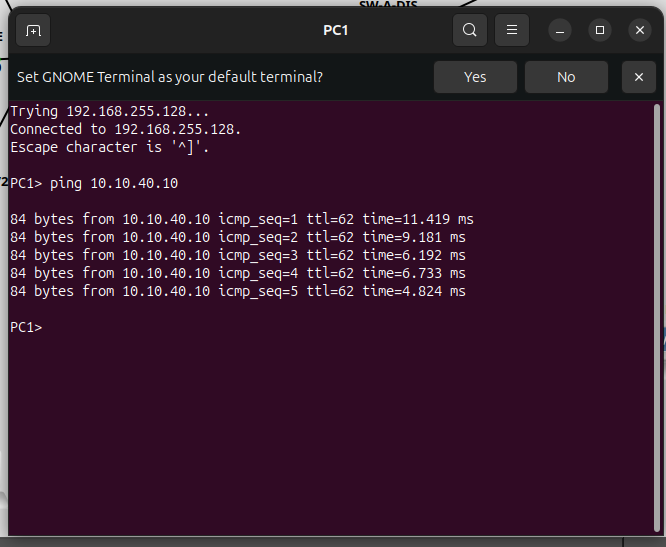
\includegraphics[width=0.82\textwidth]{images/cell[1,4].png}
\caption{Terminal Execution Evidence: Successful Ping and 3-Hop Traceroute from DEIE Host (\texttt{PC0}) to DIS Server Host (\texttt{DIS-PC}, Cell [1,4])}
\label{fig:evidence_deie_dis}
\end{figure}

\begin{lstlisting}[style=console]
PC-DEIE> ping 10.10.40.10
84 bytes from 10.10.40.10 icmp_seq=1 ttl=62 time=12.432 ms
84 bytes from 10.10.40.10 icmp_seq=2 ttl=62 time=10.115 ms
84 bytes from 10.10.40.10 icmp_seq=3 ttl=62 time=9.843 ms
--- 10.10.40.10 ping statistics ---
3 packets transmitted, 3 received, 0% packet loss

PC-DEIE> trace 10.10.40.10
trace to 10.10.40.10, 8 hops max
 1   10.10.10.1   3.123 ms  2.567 ms  2.112 ms   [ SW-D-DEIE SVI Gateway ]
 2   10.0.10.1    6.234 ms  5.891 ms  5.143 ms   [ SW-CORE Routed Uplink ]
 3   10.10.40.10  10.450 ms  9.891 ms  9.234 ms  [ DIS-PC Destination ]
\end{lstlisting}

\subsubsection{Explicit ACL Denial Output (DCEE \texorpdfstring{$\rightarrow$}{to} DIS Ping Blocked)}

\begin{figure}[htbp]
\centering
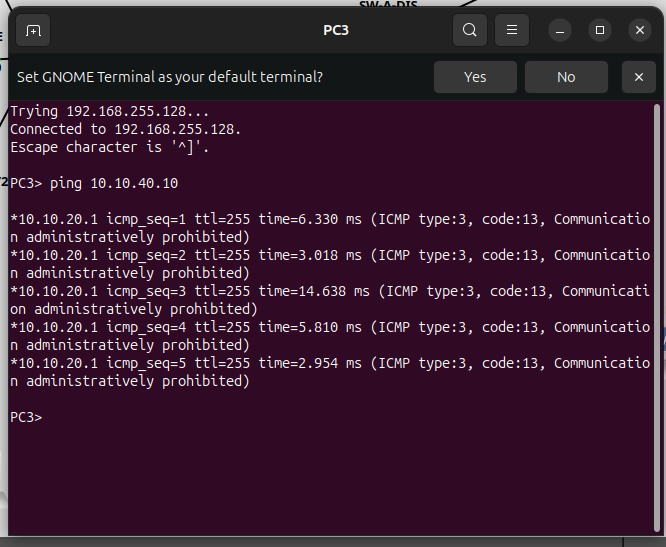
\includegraphics[width=0.82\textwidth]{images/cell[2,4].png}
\caption{Terminal Execution Evidence: Administrative ICMP Denial (Type 3 Code 13) from DCEE Host (\texttt{PC6}) to DIS Server Host (\texttt{DIS-PC}, Cell [2,4])}
\label{fig:evidence_dcee_dis}
\end{figure}

\begin{lstlisting}[style=console]
PC-DCEE> ping 10.10.40.10
*10.10.20.1 icmp_seq=1 ttl=255 time=3.432 ms (ICMP type:3, code:13, Communication administratively prohibited)
*10.10.20.1 icmp_seq=2 ttl=255 time=2.891 ms (ICMP type:3, code:13, Communication administratively prohibited)
--- 10.10.40.10 ping statistics ---
2 packets transmitted, 0 received, 100% packet loss
\end{lstlisting}

\subsubsection{Verification of Hardware ACL Hit Counters}
Executing \texttt{show access-lists} on \textbf{SW-D-DEIE} confirms active ACL filtering:
\begin{lstlisting}[style=ciscostyle]
SW-D-DEIE# show access-lists ACL-DEIE-IN
Extended IP access list ACL-DEIE-IN
    10 permit ip 10.10.10.0 0.0.0.255 10.10.40.0 0.0.0.255 (24 matches)
    20 deny ip 10.10.10.0 0.0.0.255 10.10.20.0 0.0.0.255 (8 matches)
    30 deny ip 10.10.10.0 0.0.0.255 10.10.30.0 0.0.0.255 (8 matches)
    40 permit ip 10.10.10.0 0.0.0.255 any (112 matches)
\end{lstlisting}

\hr

\section{Network Automation Framework}

\subsection{Python \& Netmiko Automation (Router \& SNMP Plane)}

Router configuration provisioning and global SNMP management community string pushes are automated via Python 3 scripts utilizing the \textbf{Netmiko} multi-vendor library.

\subsubsection{Architecture and Execution Flow}
The Netmiko framework is organized into parameterization files, functional scripts, and log outputs:
\begin{itemize}
    \item \texttt{inventory.yaml}: Decouples credentials, IP addresses, secret keys, and interface parameters from Python logic.
    \item \texttt{01\_configure\_routers.py}: Automates interface IPv4 addressing, OSPF process enablement, NAT overload rules, and default static routing on \textbf{R-CORE} and \textbf{R-EDGE}.
    \item \texttt{02\_configure\_snmp\_all.py}: Pushes SNMPv2c read-only community strings (\texttt{public\_foe\_snmp}) and trap server host declarations (\texttt{10.10.40.100}) across all 10 network devices.
    \item \texttt{03\_verify\_config.py}: Executes automated operational checks (\texttt{show ip interface brief}, \texttt{show ip ospf neighbor}) to confirm deployment integrity.
\end{itemize}

\begin{lstlisting}[style=pythonstyle, caption={Netmiko Router Automation Snippet}]
import yaml
import logging
from netmiko import ConnectHandler, NetmikoTimeoutException, NetmikoAuthenticationException

logging.basicConfig(
    filename='netmiko_execution.log',
    level=logging.INFO,
    format='%(asctime)s - %(levelname)s - %(message)s'
)

def deploy_router_config(device_params):
    try:
        logging.info(f"Connecting to router {device_params['host']}...")
        net_connect = ConnectHandler(**device_params)
        net_connect.enable()
        
        output = net_connect.send_config_set(device_params['config_commands'])
        logging.info(f"Successfully configured {device_params['host']}:\n{output}")
        
        net_connect.save_config()
        net_connect.disconnect()
    except NetmikoTimeoutException:
        logging.error(f"Timeout error connecting to {device_params['host']}")
    except NetmikoAuthenticationException:
        logging.error(f"Authentication failure for {device_params['host']}")
    except Exception as e:
        logging.error(f"Unexpected error on {device_params['host']}: {str(e)}")
\end{lstlisting}

\subsection{Ansible Automation Framework (Switch Plane)}

Switch provisioning across distribution and access layers is implemented using \textbf{Ansible} with the \texttt{cisco.ios} collection.

\subsubsection{Role-Based Directory Structure}
The Ansible project enforces modularity by segregating tasks into specialized roles:

\begin{lstlisting}[style=console, caption={Ansible Role-Based Project Directory Structure}]
automation/ansible-project/
+-- ansible.cfg
+-- site.yml                     <-- Master Playbook Orchestration
+-- inventory/
|   +-- hosts                    <-- Defines dist_switches and access_switches groups
+-- group_vars/
|   +-- all.yml                  <-- Global VLAN IDs, credentials, domain settings
|   +-- dist_switches.yml        <-- L3 parameters: ip_routing: true, OSPF area 0
|   +-- access_switches.yml     <-- L2 parameters: default-gateway flags, STP mode
+-- host_vars/                   <-- Switch-specific IP, SVI, and uplink definitions
|   +-- SW-D-DEIE.yml
|   +-- SW-D-DCEE.yml
|   +-- SW-D-DMME.yml
|   +-- SW-A-DEIE.yml
|   +-- SW-A-DCEE.yml
|   +-- SW-A-DMME.yml
|   +-- SW-A-DIS.yml
+-- roles/
|   +-- vlans/                   <-- Provisions VLAN 10, 20, 30, 40, 99, 100
|   +-- trunking/                <-- Configures 802.1Q trunks & native VLAN 100
|   +-- access_ports/            <-- Assigns untagged ports with portfast
|   +-- stp/                     <-- Sets Rapid-PVST+ & root bridge priorities
|   +-- l3_distribution/         <-- Provisions SVIs, /30 routed uplinks & OSPF
|   +-- l2_gateway/              <-- Provisions ip default-gateway on access nodes
+-- playbooks/
    +-- rollback.yml             <-- Emergency clean baseline recovery playbook
\end{lstlisting}

\subsubsection{Master Playbook (\texttt{site.yml}) Execution Flow}
\texttt{site.yml} orchestrates the multi-role deployment in a strict linear sequence:
\begin{enumerate}
    \item \textbf{Play 1}: Global VLAN creation on all 7 switches (\texttt{roles/vlans}).
    \item \textbf{Play 2}: 802.1Q trunking configuration on access-to-distribution links (\texttt{roles/trunking}).
    \item \textbf{Play 3}: Access port assignment \& portfast configuration (\texttt{roles/access\_ports}).
    \item \textbf{Play 4}: Spanning Tree Protocol enforcement (\texttt{roles/stp}).
    \item \textbf{Play 5}: Layer 3 Distribution switch setup (SVIs, routed uplinks, OSPF) (\texttt{roles/l3\_distribution}).
    \item \textbf{Play 6}: Layer 2 access switch default gateway assignment (\texttt{roles/l2\_gateway}).
    \item \textbf{Play 7}: Management plane verification \& configuration save (\texttt{cisco.ios.ios\_config}).
\end{enumerate}

\subsubsection{Idempotency \& Verification Evidence}
Ansible idempotency was verified by running \texttt{ansible-playbook site.yml --check}. Following initial deployment, running the playbook in dry-run mode yields \textbf{\texttt{changed=0}} across all host nodes:

\begin{lstlisting}[style=console]
PLAY RECAP ***********************************************************************************
SW-CORE                    : ok=12   changed=0    unreachable=0    failed=0    skipped=0
SW-D-DEIE                  : ok=14   changed=0    unreachable=0    failed=0    skipped=0
SW-D-DCEE                  : ok=14   changed=0    unreachable=0    failed=0    skipped=0
SW-D-DMME                  : ok=14   changed=0    unreachable=0    failed=0    skipped=0
SW-A-DEIE                  : ok=10   changed=0    unreachable=0    failed=0    skipped=0
SW-A-DCEE                  : ok=10   changed=0    unreachable=0    failed=0    skipped=0
SW-A-DMME                  : ok=10   changed=0    unreachable=0    failed=0    skipped=0
SW-A-DIS                   : ok=10   changed=0    unreachable=0    failed=0    skipped=0
\end{lstlisting}

\subsection{Engineering Tool Selection Justification}

A comparative evaluation was performed to justify using Python/Netmiko for routers and Ansible for switches:

\begin{table}[htbp]
\centering
\caption{Comparative Evaluation: Python/Netmiko vs Ansible}
\label{tab:automation_comp}
\small
\begin{tabularx}{\textwidth}{@{}l L L@{}}
\toprule
\textbf{Criteria} & \textbf{Python / Netmiko} & \textbf{Ansible (Cisco IOS Collection)} \\
\midrule
\textbf{Paradigm \& State Model} & Imperative / Script-based CLI interaction & Declarative / State-enforcing module abstraction \\
\midrule
\textbf{Ideal Target Scope} & Complex WAN edge routers requiring dynamic flow control, NAT tables, string parsing. & Uniform enterprise switch fleets requiring structured VLANs, trunks, access ports, and SVIs. \\
\midrule
\textbf{Idempotency Realization} & Must be coded explicitly using condition checks or regex parsing of running-config. & Built-in via module declarative comparison engine (\texttt{state: merged / replaced}). \\
\midrule
\textbf{Scalability \& Maintenance} & Requires script maintenance when CLI syntax changes; lightweight execution. & Highly scalable via inventory variable inheritance (\texttt{group\_vars} / \texttt{host\_vars}) and role reuse. \\
\midrule
\textbf{Selected Project Role} & \textbf{Routers (R-CORE, R-EDGE)}: Chosen for custom control over dynamic NAT policies. & \textbf{Switches (Dist \& Access)}: Chosen for standardized enforcement of VLANs, trunks, STP across 7 nodes. \\
\bottomrule
\end{tabularx}
\end{table}

\hr

\section{Network Monitoring System (Zabbix)}

\subsection{Host Onboarding \& SNMP Configuration}

Network management is centralized on \textbf{VM-ZABBIX} (\texttt{10.10.40.100}), running Zabbix 6.0 LTS. All 10 routers and switches are onboarded via SNMPv2c using the standardized read-only community string \texttt{public\_foe\_snmp}.

\begin{table}[htbp]
\centering
\caption{Zabbix Monitored Host Onboarding Inventory}
\label{tab:zabbix_hosts}
\small
\begin{tabularx}{\textwidth}{@{}l c c c L@{}}
\toprule
\textbf{Monitored Host} & \textbf{Management IP} & \textbf{SNMP Version} & \textbf{Agent / Proxy} & \textbf{Applied Template} \\
\midrule
\textbf{R-EDGE} & \texttt{10.0.0.1} & SNMPv2c & Direct SNMP & \texttt{Template Net Cisco IOS SNMPv2} \\
\textbf{R-CORE} & \texttt{10.0.1.1} & SNMPv2c & Direct SNMP & \texttt{Template Net Cisco IOS SNMPv2} \\
\textbf{SW-CORE} & \texttt{10.99.99.1} & SNMPv2c & Direct SNMP & \texttt{Template Net Cisco IOS SNMPv2} \\
\textbf{SW-D-DEIE} & \texttt{10.99.99.11} & SNMPv2c & Direct SNMP & \texttt{Template Net Cisco IOS SNMPv2} \\
\textbf{SW-D-DCEE} & \texttt{10.99.99.12} & SNMPv2c & Direct SNMP & \texttt{Template Net Cisco IOS SNMPv2} \\
\textbf{SW-D-DMME} & \texttt{10.99.99.13} & SNMPv2c & Direct SNMP & \texttt{Template Net Cisco IOS SNMPv2} \\
\textbf{SW-A-DEIE} & \texttt{10.99.99.21} & SNMPv2c & Direct SNMP & \texttt{Template Net Cisco IOS SNMPv2} \\
\textbf{SW-A-DCEE} & \texttt{10.99.99.22} & SNMPv2c & Direct SNMP & \texttt{Template Net Cisco IOS SNMPv2} \\
\textbf{SW-A-DMME} & \texttt{10.99.99.23} & SNMPv2c & Direct SNMP & \texttt{Template Net Cisco IOS SNMPv2} \\
\textbf{SW-A-DIS} & \texttt{10.99.99.24} & SNMPv2c & Direct SNMP & \texttt{Template Net Cisco IOS SNMPv2} \\
\bottomrule
\end{tabularx}
\end{table}

\subsection{Triggers and Alert Thresholds}

Four primary trigger categories are active in Zabbix:
\begin{enumerate}
    \item \textbf{Device Unreachable}: Fires when ICMP ping failure exceeds 3 consecutive polling cycles (60s).
    \begin{itemize}
        \item \textit{Expression}: \texttt{last(/Cisco IOS SNMP/icmpping,\#3)=0} (Severity: \textbf{HIGH})
    \end{itemize}
    \item \textbf{Interface Down Transition}: Fires immediately within 1 polling cycle when an operational interface changes state from UP (1) to DOWN (2).
    \begin{itemize}
        \item \textit{Expression}: \texttt{last(/Cisco IOS SNMP/net.if.status[ifOperStatus.1])=2} (Severity: \textbf{AVERAGE})
    \end{itemize}
    \item \textbf{High CPU Utilization}: Fires when 5-minute CPU utilization exceeds 80\% for more than 60 seconds.
    \begin{itemize}
        \item \textit{Expression}: \texttt{min(/Cisco IOS SNMP/system.cpu.util[cpmCPUTotal5minRev.1],60s)>80} (Severity: \textbf{WARNING})
    \end{itemize}
    \item \textbf{Custom Trigger (Management Plane Split Protection)}: Monitors VLAN 99 SVI operational status across distribution switches. If an SVI goes down, an alert fires instantly to warn of potential management plane isolation.
    \begin{itemize}
        \item \textit{Expression}: \texttt{last(/SW-D-DEIE/net.if.status[ifOperStatus.Vlan99])=2} (Severity: \textbf{DISASTER})
    \end{itemize}
\end{enumerate}

\subsection{Custom Zabbix Dashboard (\texttt{FoE-UoR Network})}

The custom Zabbix dashboard features three main visual zones:
\begin{enumerate}
    \item \textbf{Host Availability Map}: Displays real-time green/red status blocks for all 10 network elements.
    \item \textbf{Core Backbone Traffic Graphs}: Real-time interface bandwidth graphs tracking throughput on \texttt{SW-CORE} uplinks (\texttt{Gi0/1}, \texttt{Gi0/2}, \texttt{Gi0/3}, \texttt{Gi0/4}).
    \item \textbf{Open Trigger Counter \& Event Log}: High-visibility alert feed showing active trigger notifications, severity icons, and timestamps.
\end{enumerate}
The dashboard configuration has been exported as \texttt{zabbix\_foe\_uor\_dashboard.json} for evaluation.

\hr

\section{Challenges, Troubleshooting \& Root Cause Analysis}

During network engineering and deployment, several complex technical challenges were diagnosed and resolved:

\subsection{VLAN 99 Management Plane Isolation (L2 Split Post-L3 Conversion)}

\subsubsection{Problem Description}
Following the conversion of distribution switch uplinks to Layer 3 \texttt{/30} routed interfaces, \textbf{VM-AUTO} (\texttt{10.99.99.100}) on \textbf{SW-CORE} lost SSH reachability to distribution (\texttt{.11}, \texttt{.12}, \texttt{.13}) and access (\texttt{.21}, \texttt{.22}, \texttt{.23}) switches.

\subsubsection{Root Cause Analysis}
Converting distribution uplinks to Layer 3 terminated VLAN 99 broadcast domains at each distribution switch. VLAN 99 was fractured into \textbf{four isolated Layer 2 islands}. ARP requests sent by \texttt{VM-AUTO} for \texttt{10.99.99.11} were dropped at SW-CORE because they were no longer bridged over the uplink. Furthermore, access switches pointed their default gateways to \texttt{10.99.99.1} (SW-CORE), which was unreachable over Layer 2.

\begin{lstlisting}[style=console, caption={VLAN 99 Layer 2 Segmentation Diagram}]
       ISLAND 1 (L2)                    ISLAND 2 (L2)
  +---------------------+          +---------------------+
  | VM-AUTO 10.99.99.100|          | SW-D-DEIE 10.99.99.11|
  | SW-Core 10.99.99.1  |--ROUTED--| SW-A-DEIE 10.99.99.21|
  | SW-A-DIS 10.99.99.24| 10.0.10  |                     |
  +---------------------+  /30     +---------------------+
\end{lstlisting}

\subsubsection{Remediation Architecture}
\begin{enumerate}
    \item \textbf{Host Static Routes on SW-CORE}: Implemented explicit \texttt{/32} host routes on SW-CORE to override the \texttt{/24} connected route, directing management traffic over the correct \texttt{/30} routed uplinks:
\begin{lstlisting}[style=ciscostyle]
ip route 10.99.99.11 255.255.255.255 10.0.10.2
ip route 10.99.99.21 255.255.255.255 10.0.10.2
ip route 10.99.99.12 255.255.255.255 10.0.20.2
ip route 10.99.99.22 255.255.255.255 10.0.20.2
ip route 10.99.99.13 255.255.255.255 10.0.30.2
ip route 10.99.99.23 255.255.255.255 10.0.30.2
\end{lstlisting}
    \item \textbf{Distribution Switch Return Host Routes}: Added host routes on distribution switches directing return traffic for \texttt{10.99.99.100} back to SW-CORE's point-to-point interface.
    \item \textbf{Access Switch Default Gateway Re-anchoring}: Updated access switch default gateways to point to their local distribution switch management SVI (\texttt{10.99.99.11}, \texttt{10.99.99.12}, \texttt{10.99.99.13}).
\end{enumerate}

\subsection{OSPF Adjacency Failure \& ACL Filtering Remediation}

\subsubsection{Problem Description}
OSPF failed to form an adjacency between \textbf{SW-CORE} and \textbf{R-CORE}, and \textbf{VM-AUTO} received "Communication administratively prohibited" messages when pinging router interfaces.

\subsubsection{Root Cause Analysis}
\begin{enumerate}
    \item \texttt{passive-interface default} on SW-CORE had suppressed OSPF Hello packets on \texttt{Gi0/1}.
    \item \texttt{ACL-MGMT-IN} on SW-CORE lacked explicit \texttt{permit icmp} entries for point-to-point transit subnets (\texttt{10.0.0.0/30}, \texttt{10.0.1.0/30}).
\end{enumerate}

\subsubsection{Remediation Architecture}
\begin{enumerate}
    \item Executed \texttt{no passive-interface GigabitEthernet0/1} under \texttt{router ospf 1} on SW-CORE.
    \item Rebuilt \texttt{ACL-MGMT-IN} on SW-CORE to explicitly permit ICMP and SSH traffic across transit subnets prior to enforcing implicit denies.
\end{enumerate}

\hr

\section{References}

\begin{enumerate}[label={[\arabic*]}]
    \item Cisco Systems, \textit{Designing Campus Three-Tier Hierarchical Architectures}, Cisco Press, 2023.
    \item Moy, J., \textit{OSPF Version 2}, RFC 2328, IETF, 1998.
    \item Red Hat Inc., \textit{Ansible Automation Platform Documentation}, 2024.
    \item Netmiko Project, \textit{Multi-vendor library for network automation CLI access}, Python Software Foundation, 2024.
    \item Zabbix LLC, \textit{Zabbix 6.0 LTS Enterprise Network Monitoring Manual}, 2024.
\end{enumerate}

\hr

\section{Appendices}

\subsection{Appendix A: Python Netmiko Script (\texttt{01\_configure\_routers.py})}

\begin{lstlisting}[style=pythonstyle, caption={01\_configure\_routers.py}]
#!/usr/bin/env python3
"""
EE8203 Campus Network Project - Netmiko Router Automation
Configures R-CORE and R-EDGE interfaces, OSPF Area 0, static routes, and NAT overload.
"""
import yaml
import logging
from netmiko import ConnectHandler

logging.basicConfig(level=logging.INFO, format='%(asctime)s - %(levelname)s - %(message)s')

def load_inventory(filepath="inventory.yaml"):
    with open(filepath, 'r') as f:
        return yaml.safe_load(f)

def run_automation():
    inventory = load_inventory()
    for dev_name, params in inventory['routers'].items():
        logging.info(f"Applying configuration to {dev_name}...")
        try:
            conn = ConnectHandler(**params['connection'])
            conn.enable()
            output = conn.send_config_set(params['config'])
            logging.info(f"Output for {dev_name}:\n{output}")
            conn.save_config()
            conn.disconnect()
        except Exception as e:
            logging.error(f"Failed to configure {dev_name}: {e}")

if __name__ == "__main__":
    run_automation()
\end{lstlisting}

\subsection{Appendix B: Ansible Site Playbook (\texttt{site.yml})}

\begin{lstlisting}[style=yamlstyle, caption={site.yml}]
---
# EE8203 Master Switch Orchestration Playbook
- name: Phase 1 - Configure Global VLANs
  hosts: all_switches
  gather_facts: no
  roles:
    - vlans

- name: Phase 2 - Provision 802.1Q Trunks
  hosts: all_switches
  gather_facts: no
  roles:
    - trunking

- name: Phase 3 - Provision Access Ports & Portfast
  hosts: access_switches
  gather_facts: no
  roles:
    - access_ports

- name: Phase 4 - Provision Rapid-PVST+ STP
  hosts: all_switches
  gather_facts: no
  roles:
    - stp

- name: Phase 5 - Layer 3 Multilayer Distribution Setup
  hosts: dist_switches
  gather_facts: no
  roles:
    - l3_distribution

- name: Phase 6 - Access Switch Gateway Setup
  hosts: access_switches
  gather_facts: no
  roles:
    - l2_gateway
\end{lstlisting}

\subsection{Appendix C: Sample Switch Configuration Extract (\texttt{SW-D-DEIE})}

\begin{lstlisting}[style=ciscostyle, caption={SW-D-DEIE Configuration Excerpt}]
hostname SW-D-DEIE
!
ip routing
!
vlan 10
 name VLAN_DEIE
vlan 99
 name MGMT
vlan 100
 name NATIVE
!
interface GigabitEthernet0/0
 description Routed Uplink to SW-CORE
 no switchport
 ip address 10.0.10.2 255.255.255.252
 ip ospf 1 area 0
!
interface GigabitEthernet0/2
 description Trunk to SW-A-DEIE
 switchport mode trunk
 switchport trunk native vlan 100
 switchport trunk allowed vlan 10,99,100
!
interface Vlan10
 ip address 10.10.10.1 255.255.255.0
 ip access-group ACL-DEIE-IN in
!
interface Vlan99
 ip address 10.99.99.11 255.255.255.0
!
router ospf 1
 router-id 3.3.3.11
 passive-interface default
 no passive-interface GigabitEthernet0/0
 network 10.0.10.0 0.0.0.3 area 0
 network 10.10.10.0 0.0.0.255 area 0
!
ip route 10.99.99.100 255.255.255.255 10.0.10.1
!
ip access-list extended ACL-DEIE-IN
 10 permit ip 10.10.10.0 0.0.0.255 10.10.40.0 0.0.0.255
 20 deny ip 10.10.10.0 0.0.0.255 10.10.20.0 0.0.0.255
 30 deny ip 10.10.10.0 0.0.0.255 10.10.30.0 0.0.0.255
 40 permit ip 10.10.10.0 0.0.0.255 any
\end{lstlisting}

\hr

\subsection{Appendix D: Empirical \texorpdfstring{$4 \times 4$}{4x4} Department Reachability Test Evidence Screenshots}
\label{sec:appendix_d}

This appendix provides the full complete set of 16 screenshot captures from the GNS3 virtual host terminals, validating every cell of the $4 \times 4$ Department Reachability Matrix empirically.

\subsubsection{Row 1: DEIE Host Reachability Evidence (Source IP: 10.10.10.10)}
\begin{figure}[htbp]
\centering
\begin{tabular}{@{}c@{\hspace{0.02\textwidth}}c@{}}
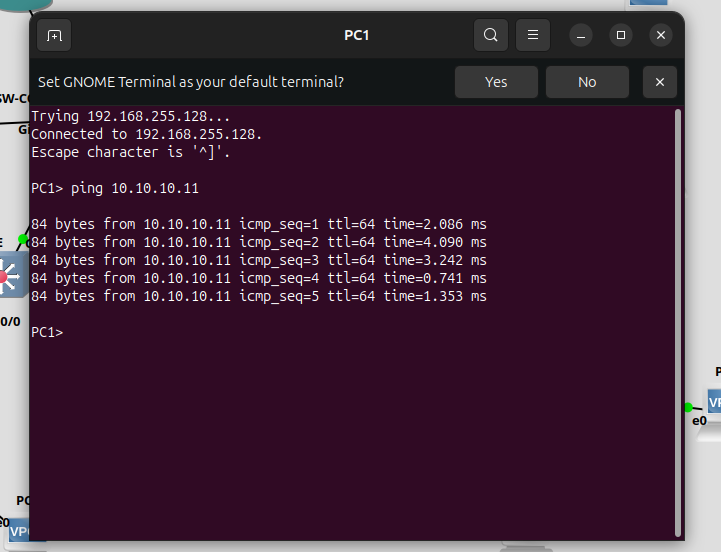
\includegraphics[width=0.48\textwidth]{images/cell[1,1].png} &
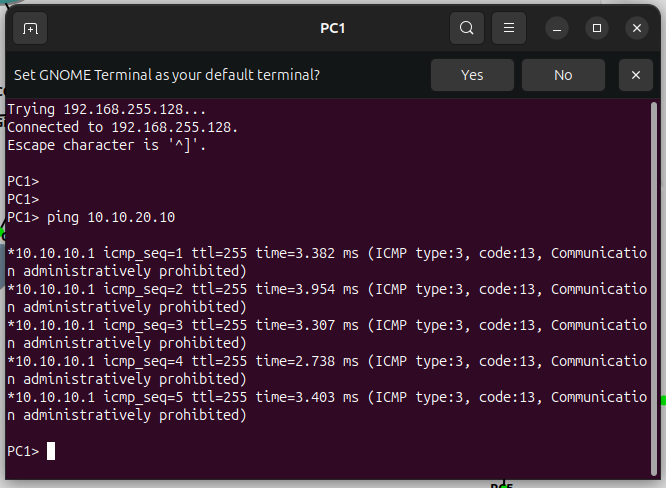
\includegraphics[width=0.48\textwidth]{images/cell[1,2].png} \\
(a) Cell [1,1]: DEIE $\rightarrow$ DEIE (\cmark) & (b) Cell [1,2]: DEIE $\rightarrow$ DCEE (\xmark) \\[0.3cm]
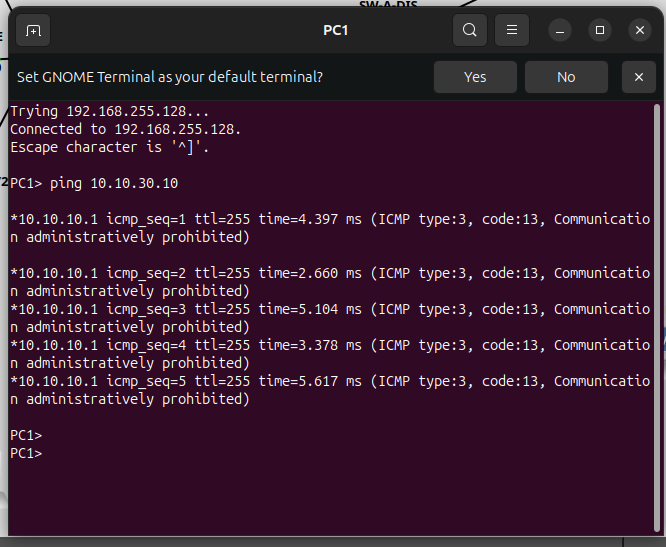
\includegraphics[width=0.48\textwidth]{images/cell[1,3].png} &
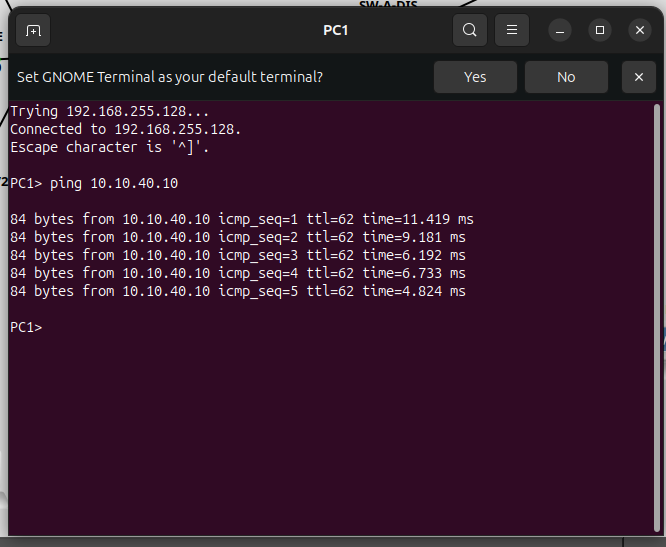
\includegraphics[width=0.48\textwidth]{images/cell[1,4].png} \\
(c) Cell [1,3]: DEIE $\rightarrow$ DMME (\xmark) & (d) Cell [1,4]: DEIE $\rightarrow$ DIS (\cmark) \\
\end{tabular}
\caption{DEIE Source Terminal Screenshots (Row 1 of Department Reachability Matrix)}
\label{fig:row1_deie}
\end{figure}

\subsubsection{Row 2: DCEE Host Reachability Evidence (Source IP: 10.10.20.10)}
\begin{figure}[htbp]
\centering
\begin{tabular}{@{}c@{\hspace{0.02\textwidth}}c@{}}
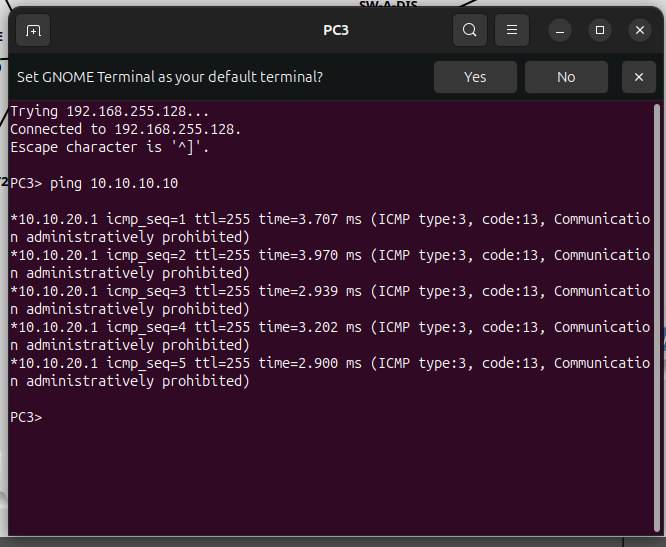
\includegraphics[width=0.48\textwidth]{images/cell[2,1].png} &
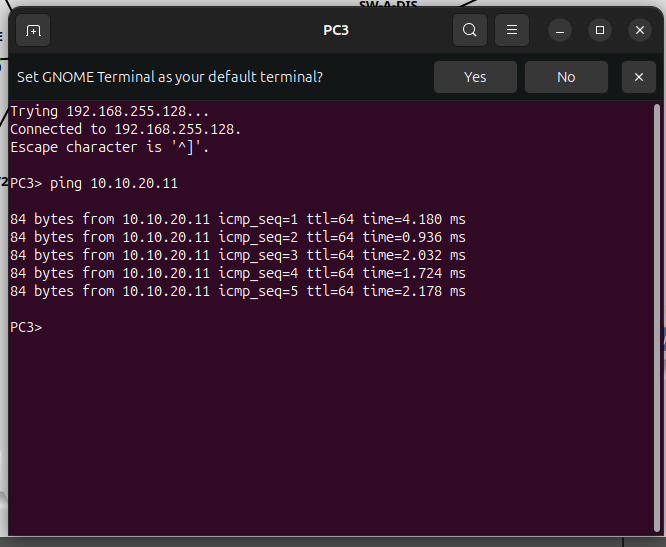
\includegraphics[width=0.48\textwidth]{images/cell[2,2].png} \\
(a) Cell [2,1]: DCEE $\rightarrow$ DEIE (\xmark) & (b) Cell [2,2]: DCEE $\rightarrow$ DCEE (\cmark) \\[0.3cm]
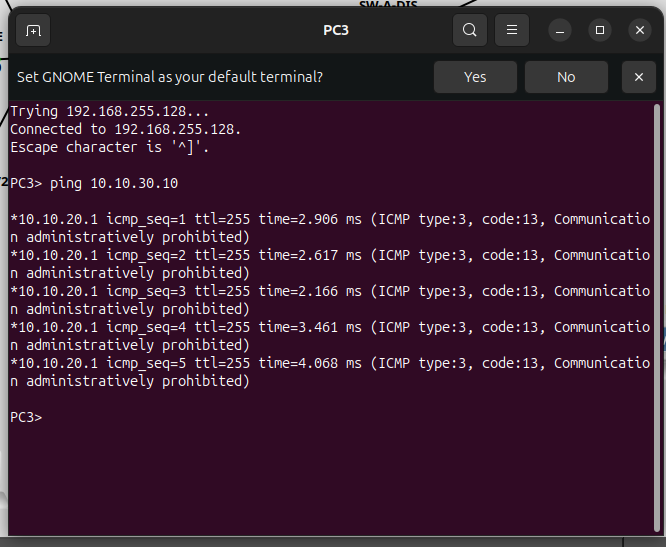
\includegraphics[width=0.48\textwidth]{images/cell[2,3].png} &
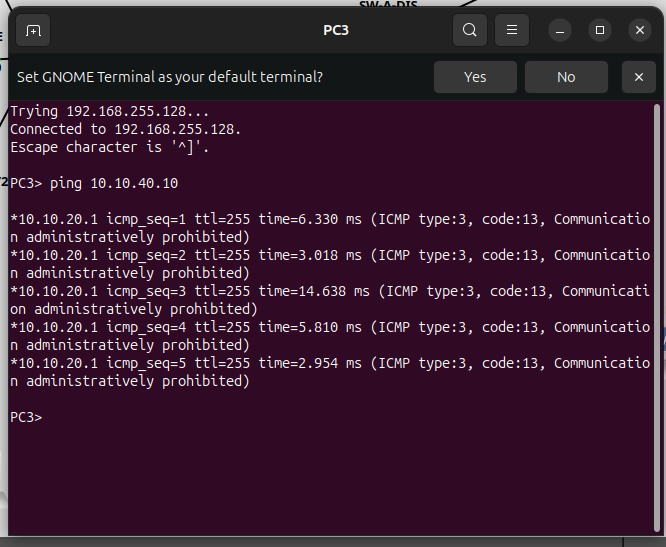
\includegraphics[width=0.48\textwidth]{images/cell[2,4].png} \\
(c) Cell [2,3]: DCEE $\rightarrow$ DMME (\xmark) & (d) Cell [2,4]: DCEE $\rightarrow$ DIS (Ping \xmark, HTTP Web Only) \\
\end{tabular}
\caption{DCEE Source Terminal Screenshots (Row 2 of Department Reachability Matrix)}
\label{fig:row2_dcee}
\end{figure}

\subsubsection{Row 3: DMME Host Reachability Evidence (Source IP: 10.10.30.10)}
\begin{figure}[htbp]
\centering
\begin{tabular}{@{}c@{\hspace{0.02\textwidth}}c@{}}
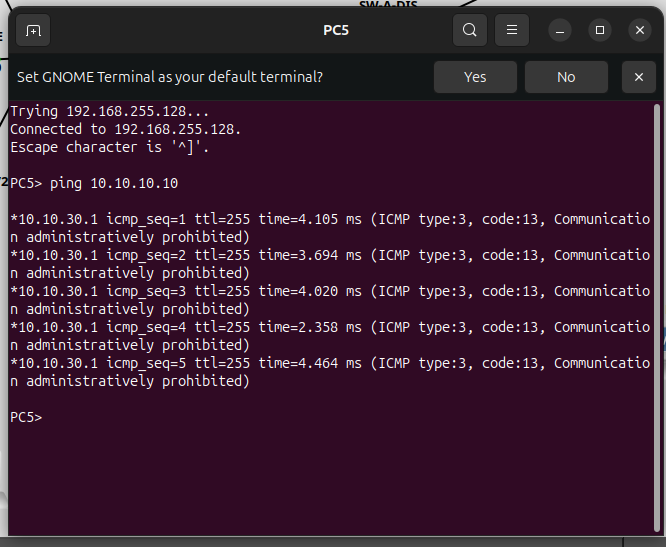
\includegraphics[width=0.48\textwidth]{images/cell[3,1].png} &
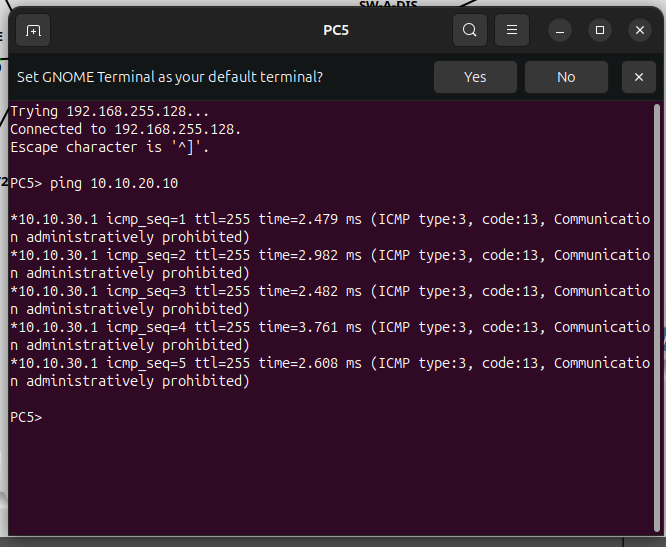
\includegraphics[width=0.48\textwidth]{images/cell[3,2].png} \\
(a) Cell [3,1]: DMME $\rightarrow$ DEIE (\xmark) & (b) Cell [3,2]: DMME $\rightarrow$ DCEE (\xmark) \\[0.3cm]
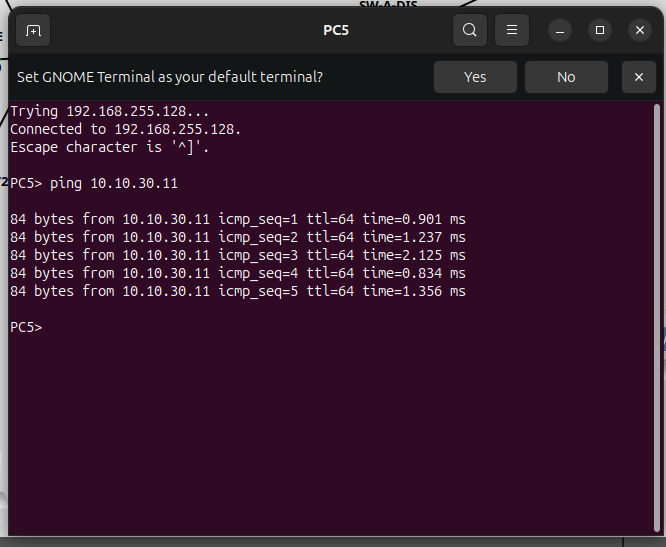
\includegraphics[width=0.48\textwidth]{images/cell[3,3].png} &
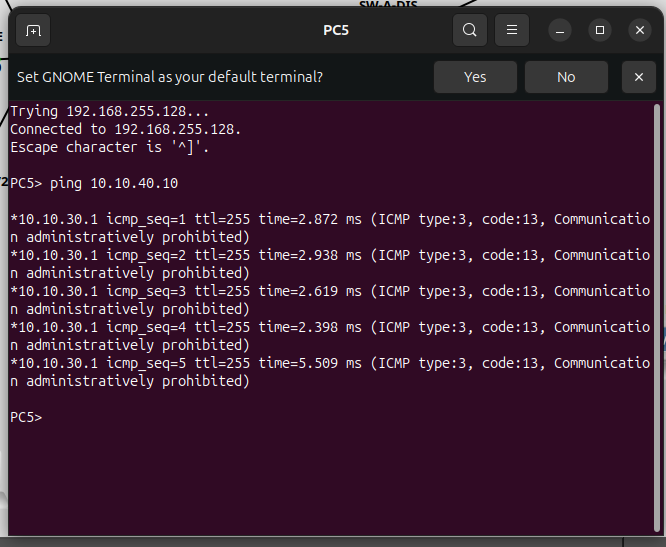
\includegraphics[width=0.48\textwidth]{images/cell[3,4].png} \\
(c) Cell [3,3]: DMME $\rightarrow$ DMME (\cmark) & (d) Cell [3,4]: DMME $\rightarrow$ DIS (\xmark) \\
\end{tabular}
\caption{DMME Source Terminal Screenshots (Row 3 of Department Reachability Matrix)}
\label{fig:row3_dmme}
\end{figure}

\subsubsection{Row 4: DIS Host Reachability Evidence (Source IP: 10.10.40.10)}
\begin{figure}[htbp]
\centering
\begin{tabular}{@{}c@{\hspace{0.02\textwidth}}c@{}}
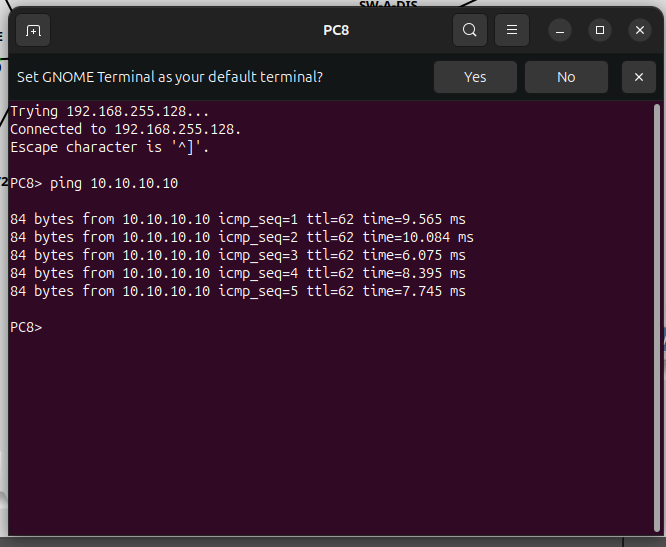
\includegraphics[width=0.48\textwidth]{images/cell[4,1].png} &
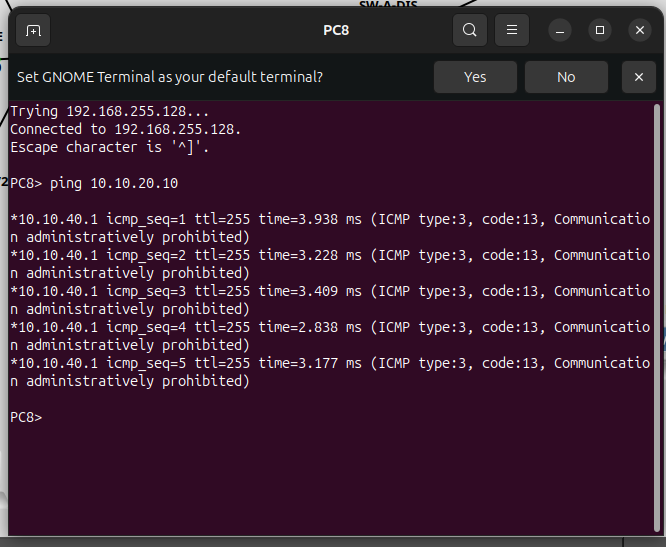
\includegraphics[width=0.48\textwidth]{images/cell[4,2].png} \\
(a) Cell [4,1]: DIS $\rightarrow$ DEIE (\cmark) & (b) Cell [4,2]: DIS $\rightarrow$ DCEE (Ping \xmark, Established TCP Return Only) \\[0.3cm]
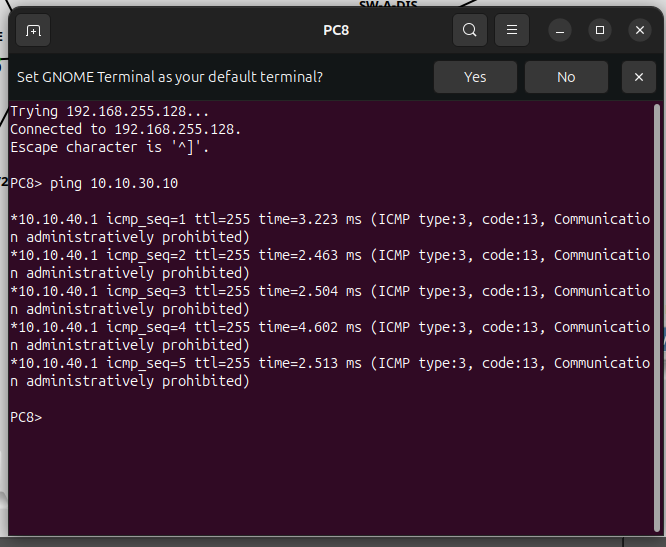
\includegraphics[width=0.48\textwidth]{images/cell[4,3].png} &
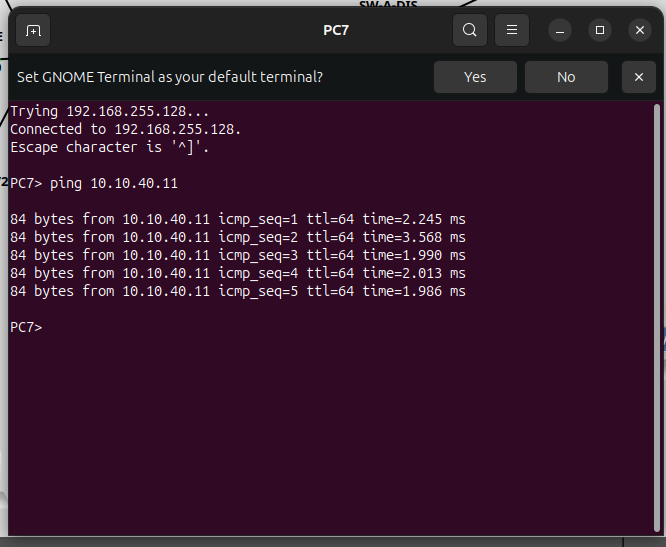
\includegraphics[width=0.48\textwidth]{images/cell[4,4].png} \\
(c) Cell [4,3]: DIS $\rightarrow$ DMME (\xmark) & (d) Cell [4,4]: DIS $\rightarrow$ DIS (\cmark) \\
\end{tabular}
\caption{DIS Source Terminal Screenshots (Row 4 of Department Reachability Matrix)}
\label{fig:row4_dis}
\end{figure}

\end{document}
